In the flux formulation, the wall-normal diffusion operator is written
in the form:
\begin{equation}
\frac{\partial}{\partial y}\left(\mu\frac{\partial u}{\partial y}\right)
\end{equation}
written here for the velocity, but the same form applies to energy and
species. However, when applied on uniform knots, the first derivative
operator yields zero for $k\Delta y=\pi$, where $\Delta y$ is the knot
spacing and $k$ is the wavenumber (this is the Nyquist frequency). This
means that the highest wavenumbers are not damped by viscous diffusion,
which is physically incorrect, and numerically problematic. To counter
this, spatial filtering will be used to eliminate the high wavenumber
components of the solution state variables.


\subsection{Cook and Cabot 8th Order Filter}
Let $F$ be a filter operator, it will be undesirable to simply apply the
filter operator to the solution at each time step, as the effect of the
filtering would then be dependent on the time discretization. To avoid
this, the filtering will be introduced through the time evolution
equations. They are of the form:
\begin{equation}
\frac{\partial u}{\partial t} = R
\end{equation}
where $R$ is the right hand side of the evolution equation for generic
conserved variable $u$. The filtering is accomplished by introducing the
filter operator as follows:
\begin{equation}
\frac{\partial u}{\partial t} = \phi(F-I)u + R,
\label{eq:time_filter}
\end{equation}
where $I$ is the identity operator and $\phi$ is a coefficient. For high
wavenumbers, for which the $F$ transfer function is nearly zero, damping
with time constant $1/\phi$ will be introduced. Making $\phi$
sufficiently large will effectively kill the high wavenumber content of
$u$.

\begin{table}[t]
\begin{center}
\begin{tabular}{llllll}
i&0&1&2&3&4\\
$a_i$&0.499825&0.666520&0.166740&0.000040&-0.000005\\
$\alpha_i$&0.500000&0.666240&0.166880
\end{tabular}
\end{center}
\caption{Coefficients for the filter in equation~\ref{eq:filter} as
 given by Cook \& Cabot (2005).}
\label{tab:coefficients}
\end{table}

The filter $F$ will be formulated as a complex discrete filter, which
will operate on the conserved variable values $u_i$ at the collocation
points $y_i$. In essence this will filter the solution in a transformed
space in $y$ in which the collocation points are uniformly spaced. The
$8^{\rm th}$ order filter used by Cook \& Cabot (2005) is proposed. It
has the form
\begin{equation}
\sum_{i=0}^2 \alpha_i(\overline u_{j+i} + \overline u_{j-i}) = \sum_{i=0}^4
 a_i(u_{j+i}+u_{j-i})
\label{eq:filter}
\end{equation}
where $\overline u_j$ are the filtered values of $u_i$. Cook \& Cabot use
values for $\alpha_i$ and $a_i$ as given in table~\ref{tab:coefficients}. The transfer
function $\hat F$of this operator, when applied in an infinite domain with
uniformly space collocation points is given by
\begin{equation}
\hat F(\hat k)=\frac{\sum_{i=0}^4a_i\cos(i\hat
 k)}{\sum_{i=0}^2\alpha_i\cos(i\hat k)}\qquad -\pi\leq\hat k\leq\pi
\label{eq:transfer}
\end{equation}
where $\hat k=k\Delta y$ and $k$ is the wavenumber. For the filter used
by Cook \& Cabot, the transfer function is shown in figure~\ref{fig:transfer}.

\begin{figure}[t]
\begin{center}
%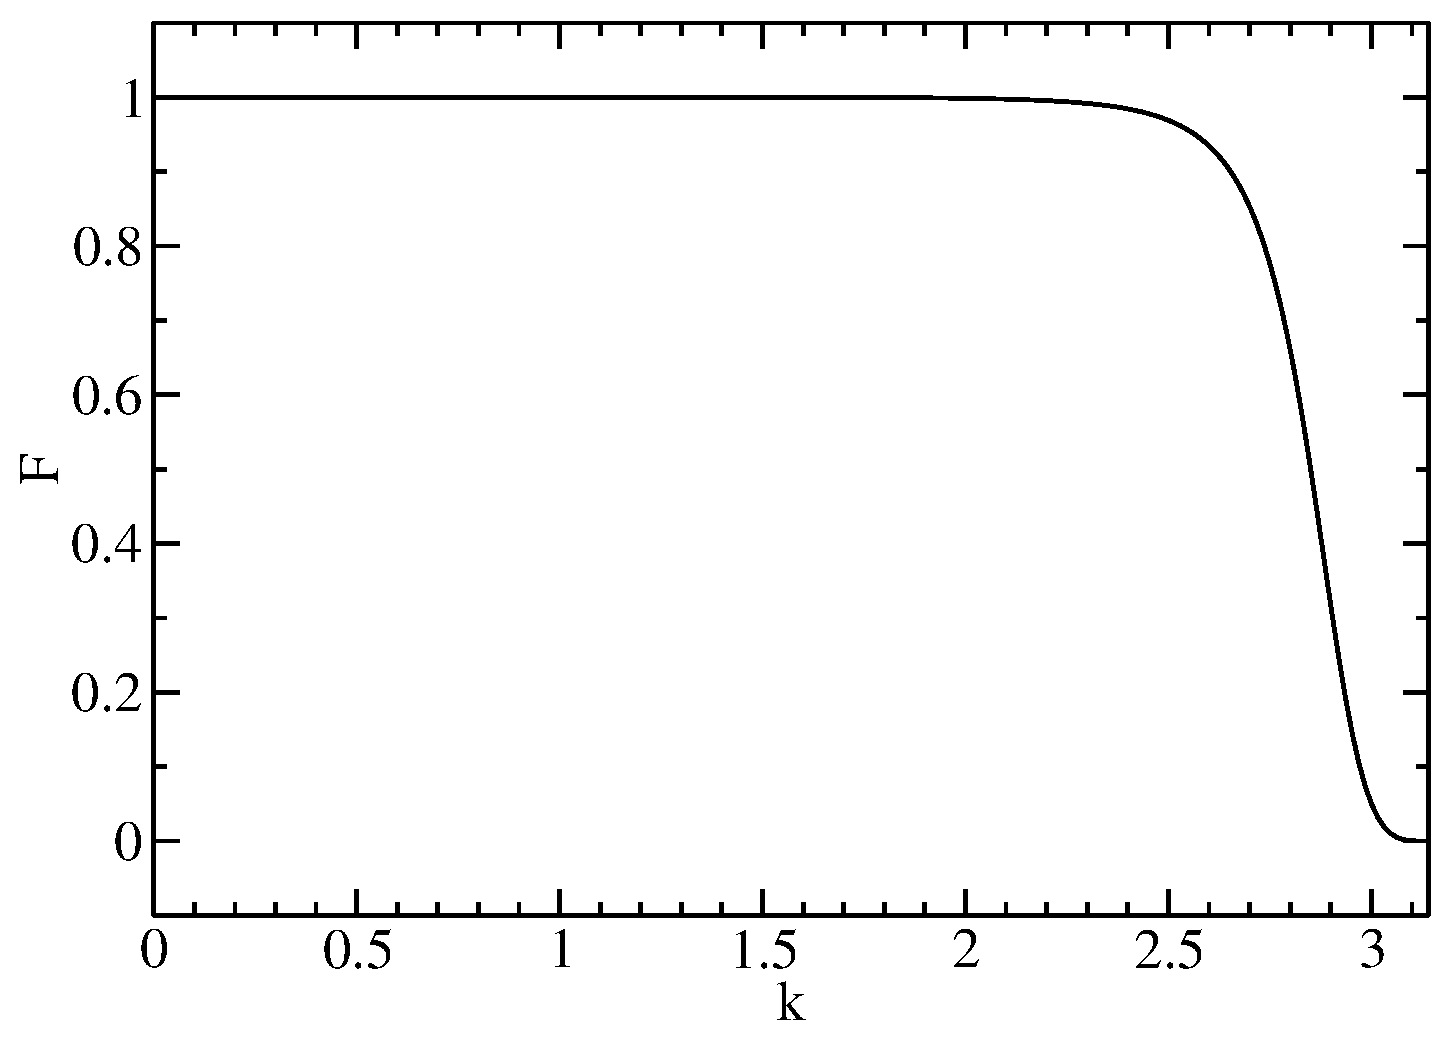
\includegraphics[width=4in]{transfer_function}
FIXME
\end{center}
 \caption{Transfer function (\ref{eq:transfer}) of the $8^{\rm th}$ order filter defined in
 (\ref{eq:filter}) and table~\ref{tab:coefficients}.}
\label{fig:transfer}
\end{figure}

There remain three details to work out: 1) the coefficients provided by
Cook \& Cabot apparently are only given to a part in $10^6$, we will
need them specified to machine precision to retain the $8^{\rm th}$
order accuracy; 2) the filter stencil is quite wide, so that for points
near the wall, the stencil will fall outside the domain; 3) the value of
$\phi$ needs to be selected. Treatment of
these issues is discussed below.

%\paragraph{Parameter Values} The filter is defined by 7 independent
Parameter Values: The filter is defined by 7 independent
parameters, which are constrained by a number of requirements:
\begin{itemize}
\item Eighth order accuracy introduced 4 linear constraints required to
      force the $0^{\rm th}$, $2^{\rm nd}$, $4^{\rm th}$ and $6^{\rm
      th}$
      order errors to zero. Odd order errors are zero by symmetry.
\item The Transfer function should be zero at $\hat k=\pi$, and ideally
      it would have a number of zero derivatives at $\pi$. The odd order
      derivatives are zero by symmetry. We can thus force the second
      derivative of the transfer function to be zero. This amounts to
      two more linear constraints
\item This leaves a 1-parameter family of transfer functions, where that
      parameter can presumably be used to adjust the location of the
      cut-off.
\end{itemize}
High precision values of the coefficients can thus be obtained by
solving the constraint equations. The order of accuracy constraints are:
\begin{eqnarray}
\sum_{i=0}^2\alpha_i&=&\sum_{i=0}^4a_i\\
\sum_{i=0}^2i^2\alpha_i&=&\sum_{i=0}^4i^2a_i\\
\sum_{i=0}^2i^4\alpha_i&=&\sum_{i=0}^4i^4a_i\\
\sum_{i=0}^2i^6\alpha_i&=&\sum_{i=0}^4i^6a_i
\end{eqnarray}
The constraints on the transfer function at $\hat k=\pi$ are:
\begin{eqnarray}
0&=&\sum_{i=0}^4a_i(-1)^i\\
0&=&\sum_{i=0}^4a_i i^2 (-1)^i
\end{eqnarray}
As it happens, all six of these equations are satisfied exactly by the
coefficients in the table. These values can thus be used, and we can defer finding other
members of the family of filters until later.

%\paragraph{Wall Treatment} There are three fairly straight-forward
Wall Treatment: There are three fairly straight-forward
approaches to filtering at the walls:
\begin{enumerate}
\item Just don't apply the filter operator for points near the
      wall. Since the filter stencil is broad, this would mean that the
      four collocation points closest to the wall would not have the
      filter applied.
\item Allow the filter kernel to spill out of the domain, with the
      external points having values obtained in some way. Victor
      suggests reflecting the solution through the wall, which ensures
      that the extended solution is continuous with continuous first
      derivatives. But the second derivatives will be discontinuous.
\item Us a one-sided high order filter at points near the wall.
\end{enumerate}
It is proposed that we start with approach (1) near the wall, and
approach (2) in the free stream. Approach (3) would need to be
formulated and will be deferred to later, in case (1) and (2)  are not
sufficient. The properties of these two approaches should be evaluated
by analyzing the eigenvalues and eigenvectors of the resulting
finite-domain $F$ operator.

%\paragraph{Selecting the value of $\phi$}
Selecting the value of $\phi$:
One wants to select $\phi$ sufficiently large so that the high
wavenumbers are effectively damped (eliminated), but not so large as to
cause significant damping for physically relevant wavenumbers. One
reasonable way to accomplish this is to note that by definition, since
this is for DNS, viscous (molecular) damping at the highest wavenumbers
is sufficient. For uniform knots and constant diffusivity, this would
suggest a value of $\phi$ of order $\pi^2\nu/\Delta y^2$, where $\nu$ is
the diffusivity (e.g. kinematic viscosity for momentum). However, this
is not the case. One possibility would thus be to make $\phi$ a function
of $y$, based on say an approximate $\nu$ representing the mean, and the
actual knot or collocation point locations. The eigen characteristics of
the resulting operator $\phi(F-I)$ in (\ref{eq:time_filter}) should also
be evaluated. Victor's experience in Comp regarding this would be useful.

\subsection{Viscous Filter}
In addition to the Cook and Cabot filter, a filter source based on the
difference between the ``real'' B-spline second derivative operator
and repeated application of the first derivative operator will be
investigated.  The primary goal of this filter choice is to avoid a
mismatch in the spectrum between the full discrete viscous operator
and the viscous contribution in the linear operator (see
\S\ref{sec:discretization} and~\S\ref{sec:implicit} for specification
of these operators).  This mismatch would make the explicit part of
the operator anti-diffusive, which can adversely effect the largest
stable time step if strong enough.  
\todo{Reference Rhys' analysis of using max vs. mean viscosity for
  reference profile in implicit operator to back this up.}

For clarity, we first describe the scheme for the following scalar
evolution equation:
%
\begin{equation*}
\pp{u}{t} = \pp{G_{visc}}{y},
\end{equation*}
% 
where $G_{visc} = \nu(u) \partial u / \partial y$.  In this case,
the ``flux-based'' B-spline collocation scheme takes the following
form
%
\begin{equation}
\label{eqn:flux_form_scalar_nofilter}
M \pp{U}{t} = D_1 M^{-1} G,
\end{equation}
% 
where $U$ is the vector of B-spline coefficients, $M$ is the mass
matrix (taking coefficients to collocation point values), $D_1$ is the
B-spline first derivative operator (taking coefficients to collocation
point derivative values).  The vector $G$ is the flux
evaluated at the collocation points, which can be written
%
\begin{equation*}
G = N D_1 U,
\end{equation*}
% 
where $N$ is the diagonal matrix containing the viscosity evaluated
at the collocation points on its diagonal.

The filter source is given by adding and subtracting different
discretizations of $\nu^* \partial^2 u / \partial y^2$
from~\eqref{eqn:flux_form_scalar_nofilter}, where $\nu^*$ is a
reference profile of the viscosity $\nu$.  Specifically,
%
\begin{equation}
\label{eqn:flux_form_scalar_wfilter}
M \pp{U}{t} = D_1 M^{-1} G + N^* (D_2 - D_1 M^{-1} D_1) U,
\end{equation}
% 
where $D_2$ is the B-spline second derivative operator and $N^*$ is
a diagonal matrix with the reference profile of $\nu$ on the diagonal.

To get the filter for the full Navier-Stokes equations, this scheme is
applied to each governing equation individually using the diagonal
linearized viscous operator derived in \S\ref{sec:implicit}.

